% $Author$ $Date$

% siminos/cgang/def2modes.tex    pdflatex 2modes
%     then:    pdflatex def2modes; bibtex def2modes; pdflatex def2modes; pdflatex def2modes
% for public version, toggle \draftfalse in setupAtlas.tex
%     (that removes all comments, the blog)

\documentclass[aip,cha,reprint,
secnumarabic,
nofootinbib, tightenlines,
nobibnotes, showkeys, showpacs,
groupedaddress
%preprint,%
%author-year,%
%author-numerical,%
]{revtex4-1}
% aip,cha,preprint,numerical, nofootinbib,
% You should use BibTeX and apsrev.bst for references
% Choosing a journal automatically selects the correct APS
% BibTeX style file (bst file), so only uncomment the line
% below if necessary.
%\bibliographystyle{apsrev4-1}

\newcommand{\version}{atlas ver. 0.1, Apr 26 2012}
% Predrag from atlas12      ver. 1.1, Apr 25 2012}

        \input setup2modes
        \input ../inputs/def
        \input def2modes

\begin{document}

\title[Low-dimensional cartography]
{Cartography of a 4-dimensional flow: A visual guide to sections and slices}

\author{Daniel Borrero-Echeverry}
\email{borrero@gatech.edu.}
\author{Keith M. Carroll}
\author{Bryce Robbins}
\author{Evangelos Siminos}
\author{Lei Zhang}
\affiliation{
 School of Physics and School of Mathematics,
 Georgia Inst. of Technology,
 Atlanta, GA  30332, USA
}

\date{\today}
%\date{18 December 2011}
%\setcounter{page}{1}

    \begin{abstract}
Symmetry reduction by the method of slices [blah blah]
the role they play in organizing chaos.
    \end{abstract}

\pacs{02.20.-a, 05.45.-a, 05.45.Jn, 47.27.ed, 47.52.+j, 83.60.Wc}
%% showpacs class option if PACS display desired
%% copied from siminos/blog/strategy.tex
% \PACS 02.20.-a \sep 05.45.-a \sep 05.45.Jn \sep 47.27.ed \sep 47.52.+j
% 02.20.-a      Group theory, mathematics
% 05.45.-a      Nonlinear dynamics and chaos
% 05.45.Jn      High-dimensional chaos
% 47.27.ed      Dynamical systems approaches (turbulent flows)
% 47.52.+j      Chaos in fluid dynamics
% 83.60.Wc      Flow instabilities
% 95.10.Fh      Chaotic dynamics

\keywords{
symmetry reduction,
equivariant dynamics,
relative equilibria,
relative periodic orbits,
slices,
moving frames
}%Use showkeys class option if keyword display desired
\maketitle

    \begin{quotation}
Today, it is possible to  [blah blah].
    \end{quotation}

\section{Introduction}
\label{s:intro}

Over the last decade, new insights into the dynamics of  [blah blah]

Our goals here are ?-fold:
(i)  [blah blah].
(ii) [blah blah].


\section{Section}
\label{s:cut}


As an example consider the  [blah blah],

%%%%%%%%%%%%%%%%%%%%%%%%%%%%%%%%%%%%%%%%%%%%%%%%%%%%%%%%%%%%%%%%%%%%%
%Predrag 2012-04-20: use Keith & Daniel's
%[x] trajectorynoarrows.png
%[ ] nearequilibriumnoarrows.png
%   make the same size as other 3, to facilitate inkscaping
%[x] bothsectionnoarrows.png
%[x] farequilibriumnoarrows.png
%
\begin{figure}
%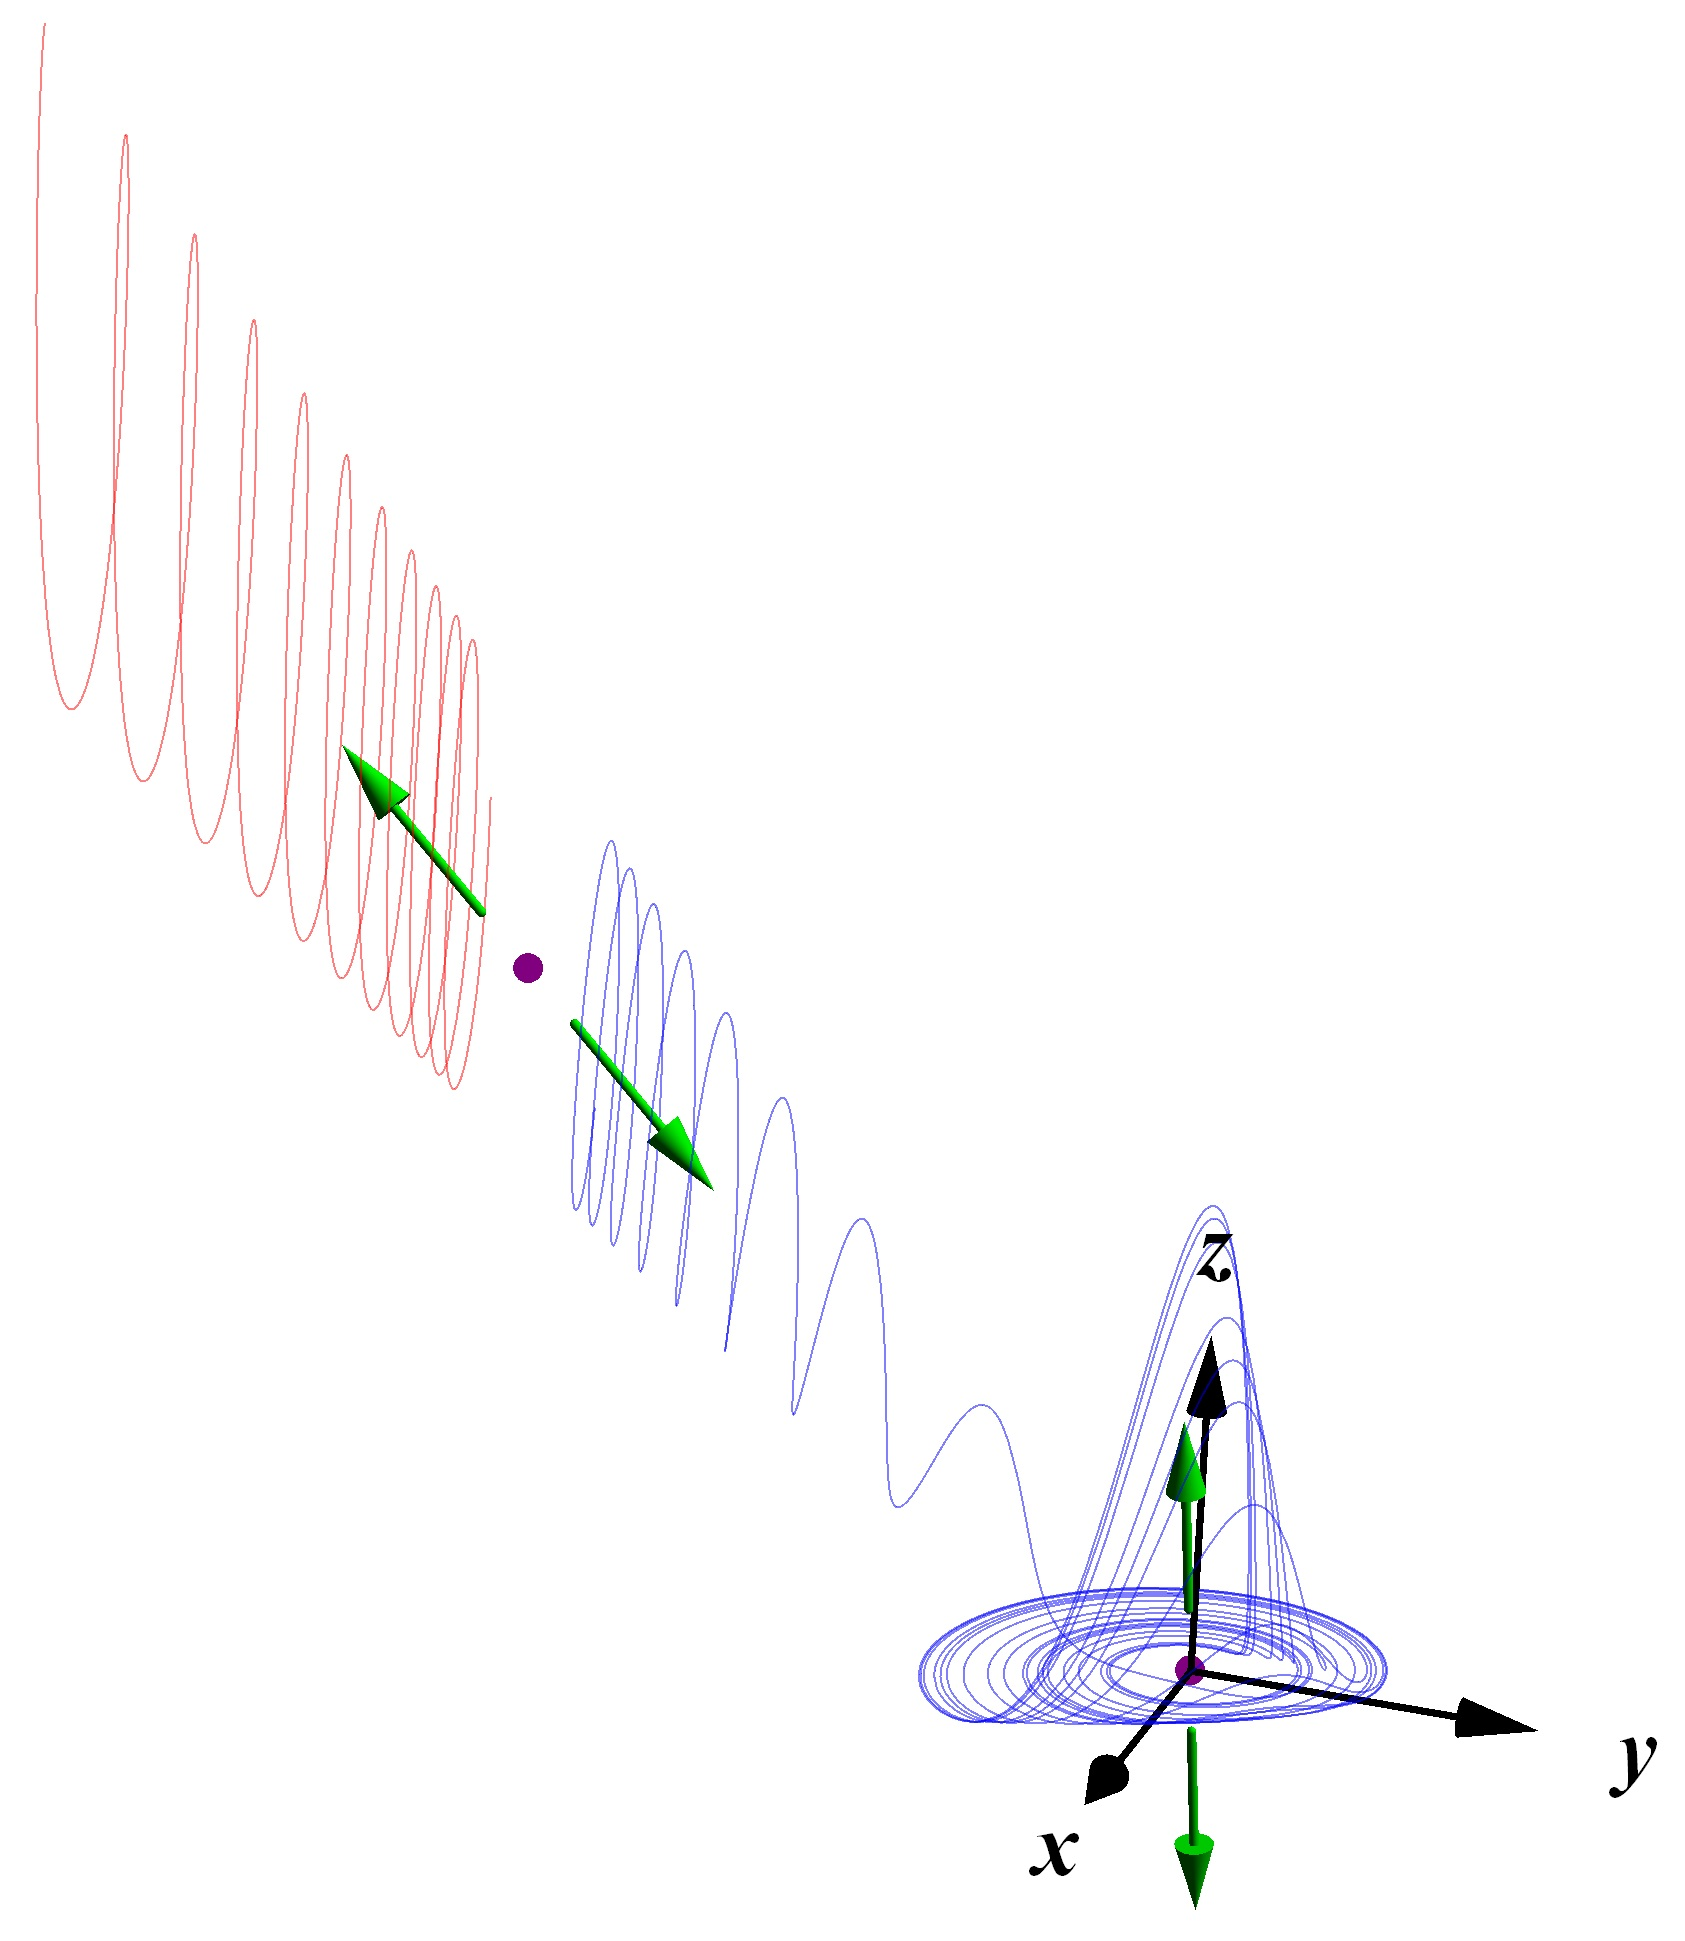
\includegraphics[width=0.28\textwidth]{RoessTrjs2}%{Rossler_Equilibria2}{RoessTrjs}%
 \begin{center}
 \setlength{\unitlength}{0.20\textwidth}
(a)
  %tried \colorbox{white}{$\slicep{}^{(-)}$} but too much white space
  \begin{picture}(1,0.8736435)%
    \put(0,0){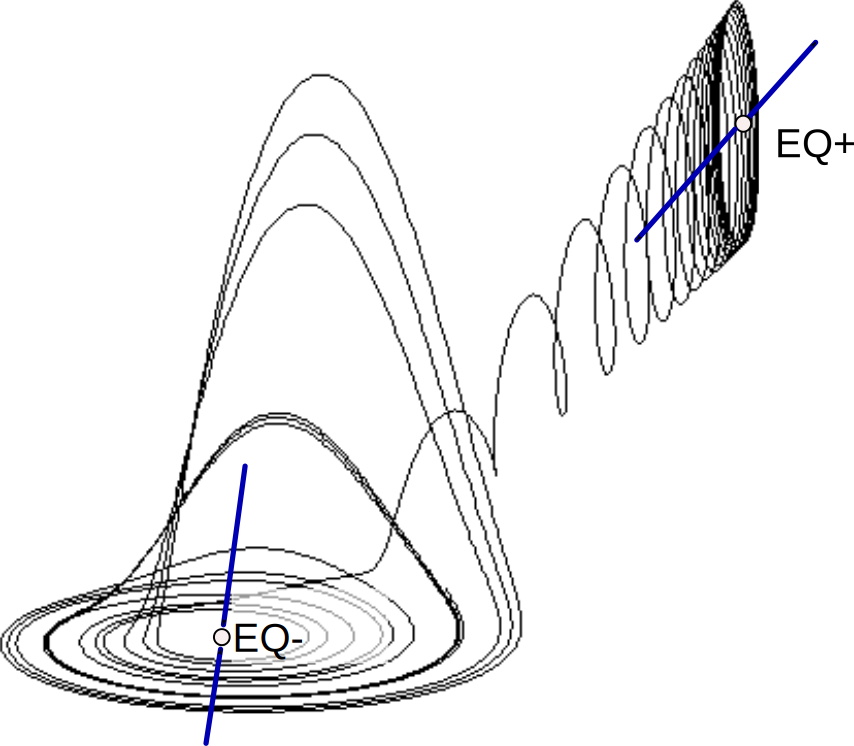
\includegraphics[width=\unitlength]{RoessTrajLbld}}%
    \put(0.27213233,0.11036704){\color[rgb]{0,0,0}\makebox(0,0)[lb]{\smash{$\slicep{}^{(-)}$}}}%
    \put(0.90759454,0.68935432){\color[rgb]{0,0,0}\makebox(0,0)[lb]{\smash{$\slicep{}^{(+)}$}}}%
  \end{picture}%
(b) %{RoessNearEq3}
  \begin{picture}(1,0.82646416)%
    \put(0,0){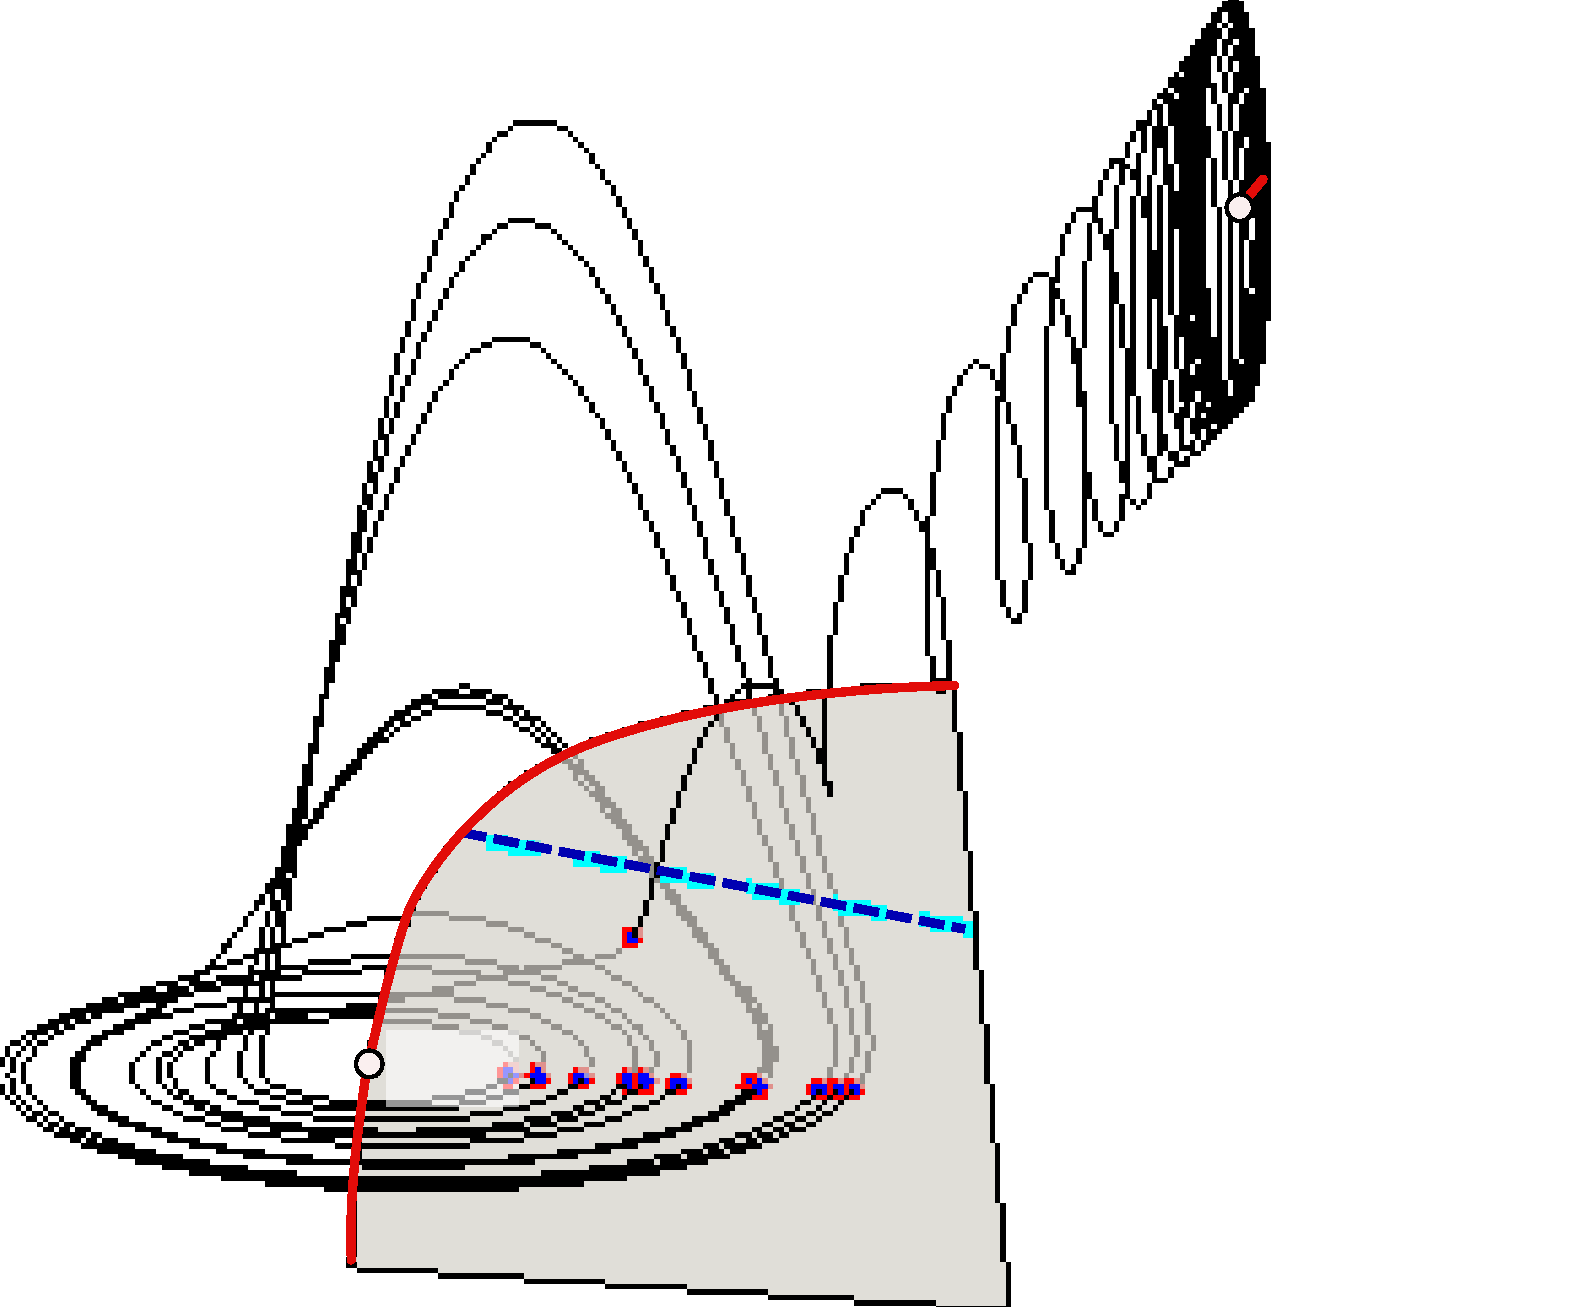
\includegraphics[width=\unitlength]{RoessNeareqLbld}}%
    \put(0.2468894,0.13781942){\color[rgb]{0,0,0}\makebox(0,0)[lb]{\smash{$\slicep{}^{(-)}$}}}%
  \end{picture}%
\\
(c)  %{RoessFarEq3}
  \begin{picture}(1,0.82646416)%
    \put(0,0){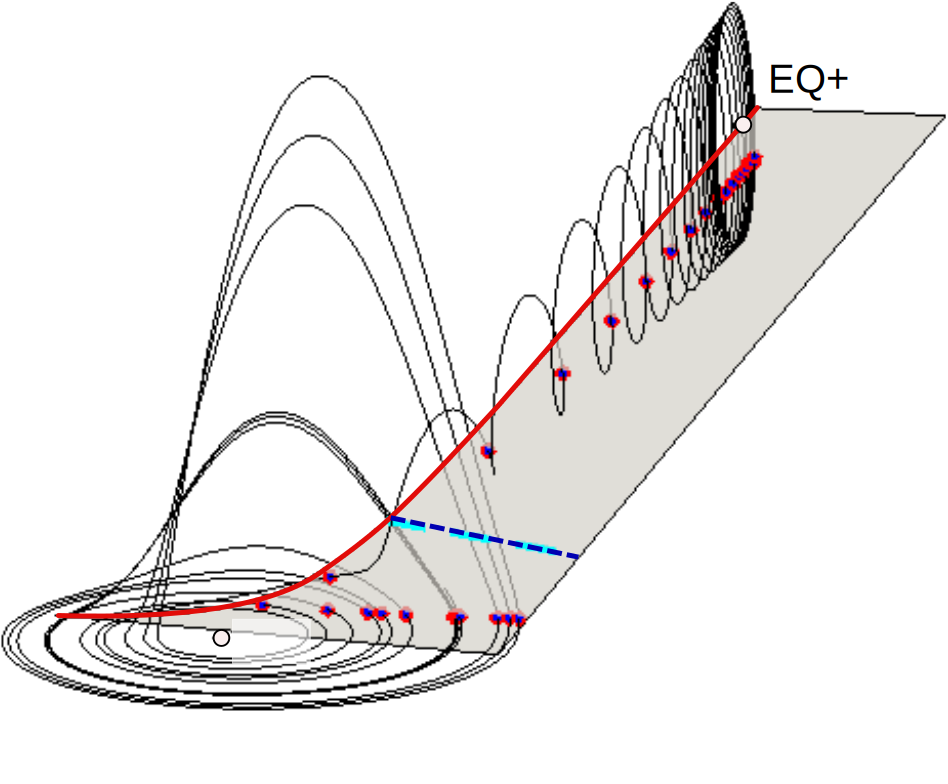
\includegraphics[width=\unitlength]{RoessFareqLbld}}%
    \put(0.81012394,0.72899125){\color[rgb]{0,0,0}\makebox(0,0)[lb]{\smash{$\slicep{}^{(+)}$}}}%
  \end{picture}%
(d)  %{RoessSctAtlas3}
  \begin{picture}(1,0.82646416)%
    \put(0,0){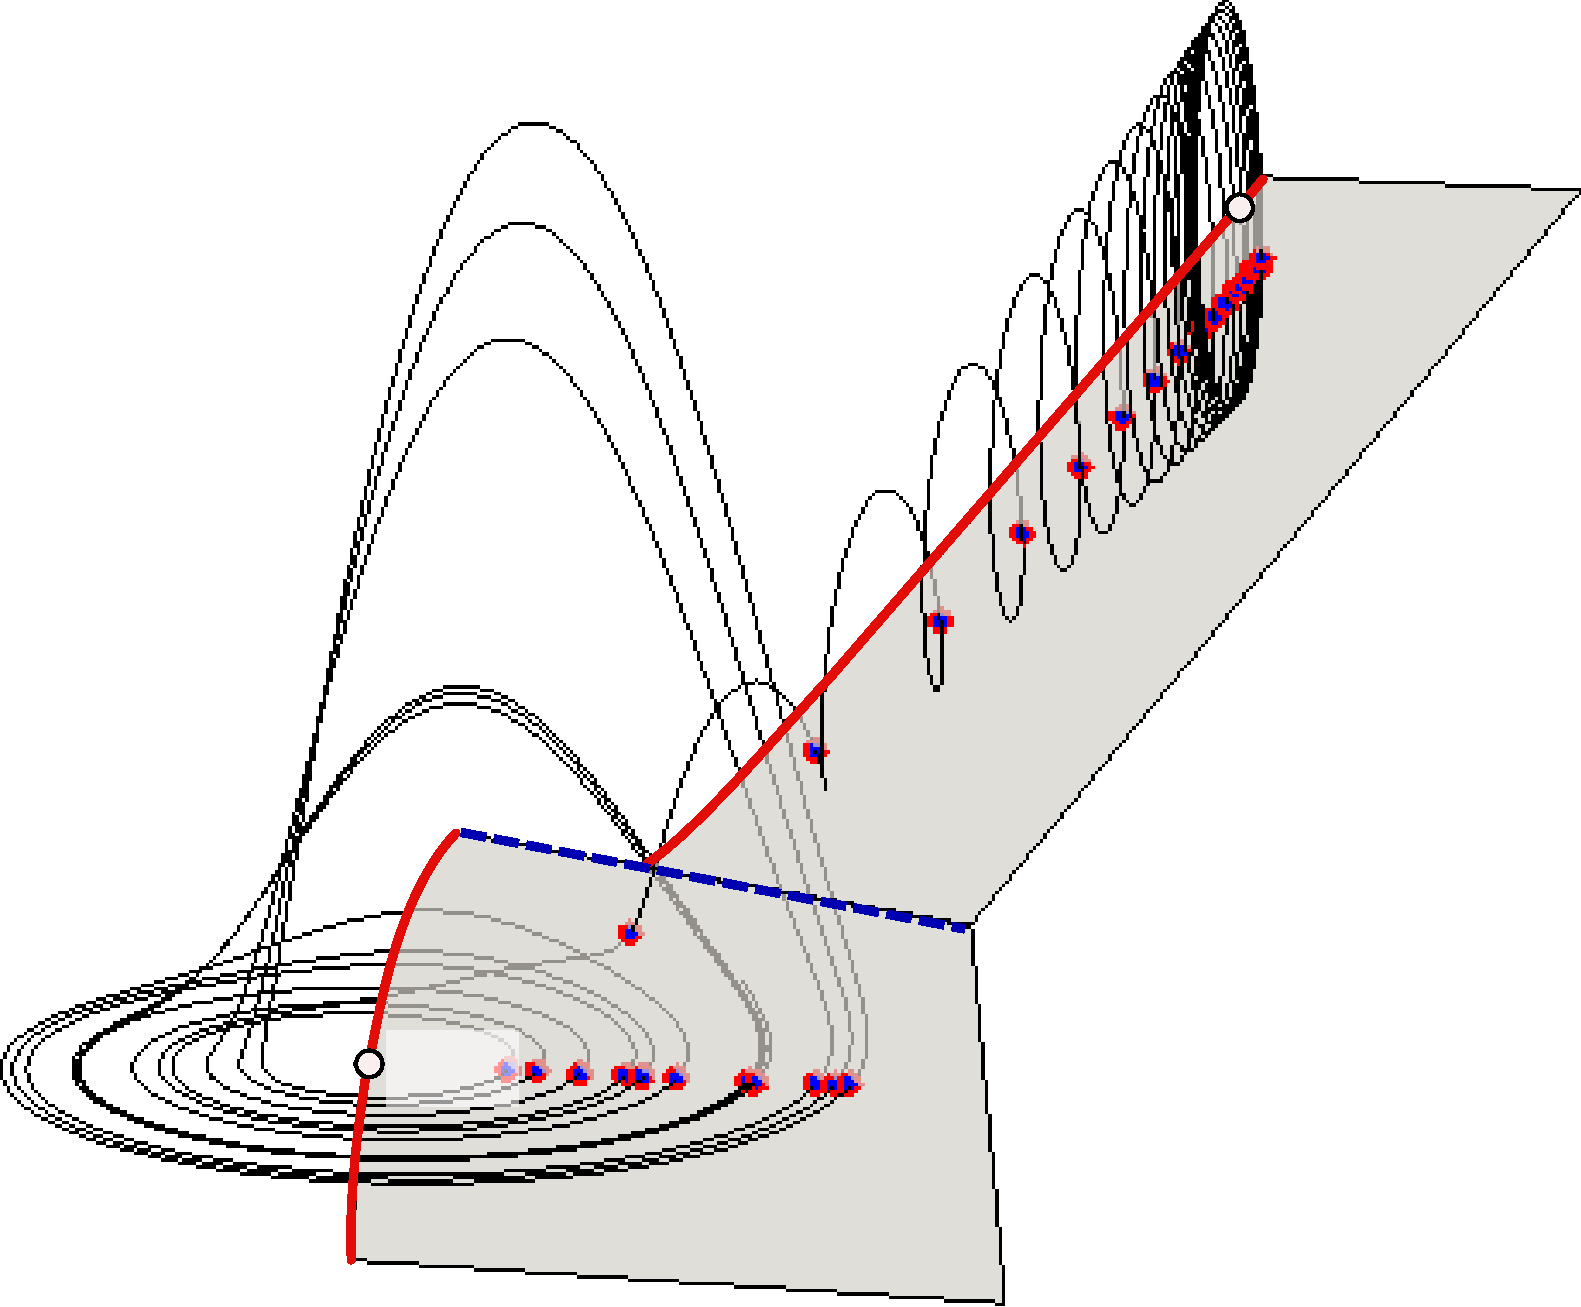
\includegraphics[width=\unitlength]{RoessBotheqLbld}}%
    \put(0.2468894,0.13781942){\color[rgb]{0,0,0}\makebox(0,0)[lb]{\smash{$\slicep{}^{(-)}$}}}%
    \put(0.81012394,0.66084196){\color[rgb]{0,0,0}\makebox(0,0)[lb]{\smash{$\slicep{}^{(+)}$}}}%
  \end{picture}%
 \end{center}
    \caption{
2-chart atlas for R\"ossler flow.
(a)
  The inner {\eqv} $\slicep{}^{(-)}$  is a (spiral-out) saddle-focus with
  a 2-dimensional unstable manifold and a 1-dimensional stable manifold.
  The outer {\eqv} $\slicep{}^{(+)}$ is a (spiral-in) saddle-focus, with
  a 2-dimensional stable manifold (basin boundary for initial conditions
  that either fall into the  chaotic attractor, or escape to infinity)
  and a 1-dimensional unstable manifold.
(b)
 Chart $\PoincS_{-}$ of the $\slicep{}^{(-)}$ neighborhood carved out of a
 \PoincSec\ plane through the inner {\eqv} $\slicep{}^{(-)}$ and its
 stable eigenvector, with \poincBord\ drawn as the solid red line.
(c)
  Chart $\PoincS_{+}$ (here viewed from below) is bounded by \poincBord\
  (solid red line) of a section through the outer {\eqv}
  $\slicep{}^{(+)}$  and its unstable eigenvector.  Note the ridge
  (dashed blue line): the chart stops at the ridge, and it does not
  intersect the strange attractor.
(d)
  A two-chart atlas of R\"ossler flow, with charts $\PoincS_{-}$ and
  $\PoincS_{+}$ oriented and combined so that the ridge (intersection of
  the two sections, indicated by the dashed blue line in the three
  figures) lies approximately between the \template s. Section
  hyperplanes beyond this ridge do not belong to the atlas.
    }
\label{fig:RoessTrjs}
\end{figure}
%%%%%%%%%%%%%%%%%%%%%%%%%%%%%%%%%%%%%%%%%%%%%%%%%%%%%%%%%%%%%%%%%%%%%

 [blah blah]

\section{Dynamics and symmetry}
\label{s:symm}
To do:

\begin{itemize}
  \item[10.8]  An $\SOn{2}$-equivariant flow with two Fourier modes
  \item[10.10] $\SOn{2}$ equivariance of the {\twoMode} system
           for infinitesimal angles.
  \item[10.11] Visualizations of the 4-dimensional {\twoMode} system
  \item[10.1?] draw a group orbit for the {\twoMode} model
  \item[10.22] {\twoMode} system in polar coordinates.
  \item[10.23] The relative equilibria of the {\twoMode} system
  \item[10.24] Plotting the relative equilibria of
           the {\twoMode} system in polar coordinates
  \item[10.25] Plotting the relative equilibria of
           the {\twoMode} system in Cartesian coordinates
  \item[10.2?] construct a 2-chart atlas for a {\twoMode} system
\end{itemize}


Armbruster, Guckenheimer and Holmes\rf{AGHO288} flow with
$\On{2}$ symmetry:
\index{Armbruster-Guckenheimer-Holmes flow}
\beq
\begin{split}
  \dot{z}_1 &=\bar{z}_1 z_2
              + z_1\left(\mu_1+ e_{11}|z_1|^2+e_{12}|z_2|^2\right) \\
  \dot{z}_2 &=\pm z_1^2
              + z_2\left(\mu_2+ e_{21}|z_1|^2+e_{22}|z_2|^2\right)
  \label{eq:2modesAGH}
\end{split}
\eeq
where $z_1,z_2\in \mathbf{C}$ and $\mu_j$ and $e_{jk}$ real parameters.
This system corresponds to the first few terms in the center manifold
reduction of a $\On{2}$-symmetric partial differential equation near a
codimension two bifurcation. It is a {\twoMode} system, so group orbits are
more interesting than for \cLf.
{\bf [2009-08-28 Predrag]} Evangelos in his thesis and
\HREF{http://chaosbook.org/projects/index.shtml\#Kohler}{Kohler} in his
\HREF{http://ChaosBook.org/projects}
     {ChaosBook.org project}
got nothing of interest out of Armbruster \etal\rf{AGHO288}. As far as we
can tell, it exhibits no chaos. I would prefer some modification of it
with $\SOn{2}$ symmetry only, and exhibiting chaos (done! see 2012-03-27
remark below). Or some version of {\twoMode} model Daniel has been playing
with which does not behave singularly. He has an unstable cycle close to
the origin that maybe does the trick.

Porter and Knobloch\rf{PoKno05}
(\HREF{http://ChaosBook.org/library/PoKno05.pdf}{click here})
write: ``Chossat\rf{Choss93} has shown that breaking the symmetry
$\On{2}$ down to $\SOn{2}$ through the addition of small terms that break
reflection symmetry generically destroys the heteroclinic cycles and
replaces them by a quasiperiodic orbit characterized by two small
frequencies, one associated with the broken heteroclinic connection and
one with a slow drift along the group orbit of translations. Ashwin
\etal\rf{AshBoMe96} showed that this perturbation must be dispersive: if
reflection symmetry is broken by adding a constant through flow the cycle
will persist.''

This shows us how to get an $\SOn{2}$-equivariant model rather than
the Armbruster, Guckenheimer and Holmes\rf{AGHO288}:
``When the reflection symmetry is broken, the coefficients in the normal
form equations are no longer forced to be real and hence can be expected
to acquire imaginary parts'', their Eq. (10). Play with that one.

 [blah blah]

Mercader and Prat\rf{MePrKn01} might
be a candidate if we decide to go with $\On{2}$ symmetry since really the
Rayleigh-Benard problem has $\On{2} \times Z_2$ symmetry and they are really
talking about breaking the $Z_2$ part. They have a reduced model, but I'm
not sure that it is chaotic.

notes on Mercader and Prat\rf{MePrKn01}.
\index{Armbruster-Guckenheimer-Holmes flow}
The effects of weak breaking of the midplane reflection symmetry on the
1:2 steady state mode interaction in Rayleigh-B\'enard convection are
discussed, with bifurcations galore, ala Knobloch. They do it for the
full PDEs, but in Sect.~4 motivate results by discussing them in the
context of $\On{2}$-equivariant amplitude equations for 1:2 mode
interactions.
We note that the Dangelmayr\rf{Dang86} and Armbruster, Guckenheimer and
Holmes\rf{AGHO288} third order in the amplitudes normal form flow with
$\On{2}$ symmetry \refeq{eq:2modesAGH} does have ratios of form $r_0/r_1$, when
rewritten in the polar form (Eq.~(4) in the paper),
\bea
   \dot{r}_1 &=& \mu_1 r_1 + a_1 r_1^3  + b_1 r_1 r_2^2
                 + c_1 r_1 r_2 \cos(\psi)\continue
   \dot{r}_2 &=& \mu_2 r_2 + a_2 r_1^2 r_2  + b_2 r_2^3
                 + c_2 r_1^2 \cos(\psi)\continue
   \dot{\theta}_1 &=&  - c_1 r_2 \sin(\psi)\,,\quad
   \dot{\theta}_2 = -e_2 + c_2 \frac{r_1^2}{r_2} \sin(\psi)
\,,
\label{eq:2modesAGpolar}
\eea
where $\psi = 2 \theta_1 - \theta_2$, and Predrag stuck in tentatively an
`$e_2$' term because something like that is needed to break $\On{2} \to
\SOn{2}$. Rewriting the angular part as $\dot{\psi} = 2 \dot{\theta_1} -
\dot{\theta_2}$:
\beq
\dot{\psi} = e_2 - \left(c_2 \frac{r_1^2}{r_2} + 2\,c_1 r_2\right) \sin(\psi)
\,.
\ee{eq:AGphase}
The equations possess pure $n = 2$ solutions but no pure $n = 1$
solutions (except for the discrete `midplane reflection' symmetry
invariant subspace?). Most solutions are `mixed modes'. I do not think we
care about the `midplane reflection' symmetry (with 5th order normal
form), so we only need \refeq{eq:2modesAGpolar} to determine the \reqva.


 [blah blah]

I'm still in favor of trying {\bf
[2012-03-27 Predrag]} Porter and Knobloch\rf{PoKno05} above, as I prefer
the most cited model. The exact 1:2 resonance ODE normal form was
treated first by  Dangelmayr\rf{Dang86} and analyzed by the more cited
Armbruster, Guckenheimer and Holmes\rf{AGHO288} and Jones and
Proctor\rf{JoPro87} (for a  general reference containing this material,
see Golubitsky \etal\rf{golubII}, ch.~XX, sect.~1), and keeps getting
cited a lot\rf{AshDang05,PoKno05,SmMoehHo05}.

Making it $\SOn{2}$-equivariant is easy, just make a coefficient complex
- I have forgotten, but that's how we got to the \cLe. If the imaginary
part is small, then you turn orbits that used to be \po s into \rpo s.
That's why {\bf [2012-03-22 Bryce]} \rpo s were nearly periodic. But
truncations of the Ginsberg-Landau equation have their market too.

Play with them both, we pick one eventually that illustrates multiple
charts better.


 [blah blah]


\begin{enumerate}
  \item
        determine \emph{numerically} the \reqva\ of the
        $\SOn{2}$-equivariant Dangelmayr {\twoMode} system in polar coordinates
\bea
   0 &=&  r_1 (\mu_1 + a_1 r_1^2  + b_1 r_1 r_2
                 + c_1 r_2 \cos(\psi))  \continue
   0 &=& \mu_2 r_2 + a_2 r_1^2 r_2  + b_2 r_2^3
                 + c_2 r_1^2 \cos(\psi)\continue
   0 &=&  e - \left(c_2 \frac{r_1^2}{r_2} + 2\,c_1 r_2\right) \sin(\psi)
\,,
\label{eq:2modesAGpolarREQV}
\eea
        Here I stuck in tentatively an `$e$' term because something like
        that is needed to break $\On{2} \to \SOn{2}$, verify that it
        really does that. The first two equations are cubic, the third one you can use
        to eliminate $\cos(\psi)$, so my guess is that there could  be up to six real
        roots, but I have not thought it through. Once you have found parameters
        for which there are interesting \reqv\ solutions, then
  \item
        compute analytically the \stabmat\ \Mvar\ in polar coordinates
  \item
        Study eigenvalues, keep playing with parameters. We would like
        -preferably- no \reqv\ to be attracting limit cycle, and several of
        the \reqva\ to be complex-pair unstable, leading to chaos, to be
        visualized and sliced in Cartesian coordinates \refeq{eq:2modesAGH}.
  \item
        If you find a nice chaotic attractors, others can join in
        constructing an atlas for it. We just need one and only one
        example with non-trivial \chartBord s and at least 2 charts.
\end{enumerate}


 [blah blah]

the $e$ added really breaks the $O(2)$ symmetry to $SO(2)$
symmetry. As rotations don't change the equations and reflections change
the sign of the last equation, adding a nonzero $e$ will break the
reflection symmetry.

By eliminating $\psi$, I got two polynomial equations of order 10. So
there are 20 complex solutions. I tried parameters $\mu_1=\mu_2=-1$,
$a_1=a_2=b_1=b_2=c_1=c_2=1$, and got 8 real solutions. All the 8
solutions I got for $(r_1,r_2)$ are $(\pm 0.537655,\pm 0.537655)$ and
$(\pm 0.980269,\pm 0.980269)$. In this case, 6 equilibria points have
only real eigenvalues, two equilibria points have complex eigenvalues
with positive real parts. Will this case work? Others please check
whether the calculation is correct or not.

 [blah blah]

By definition, $r_i \geq 0$, so you have
only two roots: $(0.537655,0.537655)$ and $(0.980269,0.980269)$. I find
it surprising that $r_1=r_2$, as equations look asymmetric in $r_i$;
might be consequence of $a_1=a_2=b_1=b_2=c_1=c_2=1$ (what value $e$? also
$e=1$?), you want to break this artificial symmetry if it is the cause. If
$r=r_1=r_2$ you have
\bea
   0 &=&  r (\mu_1 + (a_1 + b_1) r^2
                 + c_1 r \cos(\psi))  \continue
   0 &=& r (\mu_2 + (a_2 + b_2)  r^2
                 + c_2 r \cos(\psi))\continue
   0 &=&  e - r \left(c_2 + 2\,c_1\right) \sin(\psi)
\,,
\label{eq:2modesAGpolarR1R2}
\eea
which looks degenerate for your coefficient values.
There is an \eqv\ for $r_1=r_2=0$. There is a subspace $r_1=0$, $r_2 > 0$
which you can solve analytically - it my cause us some trouble. If what
you end up solving is a polynomial in $r_1$, you want to divide it with
all these known roots, see whether anything of interest is still left.

 [blah blah]

randomly chose all
the parameters and see what kinds of eigenvalues we can get. Under the
condition $r_1$ and $r_2$ being nonnegative real numbers, it seems that I
always got two equilibria points. One possible set of parameters I found
may be of interest are
$\mu_1=-1,\mu_2=-4,a_1=1,a_2=1.5,b_1=3,b_2=2.5,c_1=3,c_2=3.5,e=0.1$. The
equilibria points are $(r_1,r_2)=(0.0516508, 1.26311)$ and
$(0.467095,0.2146)$. The corresponding eigenvalues are
$(19.9398,0.8495,-11.9818)$ and $(1.5352,-4.7992+0.0327i,
-4.7992-0.0327i)$


 [blah blah]

\begin{itemize}
  \item $\REQV{}{1} = (r_1,r_2,\psi)=(0.0516508, 1.26311,?)$ and
        $\REQV{}{2} = (0.467095,0.2146,?)$
  \item their plots in the Cartesian coordinates
  \item $\dot{\theta}$ to see how slow/fast are they. $\dot{\theta}$
        might be related to 4th eigenvalue, when you go back
        to Cartesian coordinates
  \item stability eigenvalues, eigenvectors of the \eqv\ $\EQV{0}$ at
        origin, at your parameter values - if it is stable, everything
        just might fall into it and die.
  \item plots of small perturbations of the above \eqv\ and \reqva\ in
        the Cartesian coordinates to see whether the dynamics looks
        chaotic
  \item $\REQV{}{1}$: 2 large positive eigenvalues looks scary - probably
        nothing re-visits this \reqv. A mildly unstable complex pair
        would have been sweeter. You get complex eigenvalue by Hopf-bifurcating off a
        stable orbit, typically.
  \item $\REQV{}{1}$: Does either unstable eigenvalue become a complex
        eigenvalue pair in Cartesian coordinates?
  \item $\REQV{}{2}$: contracting eigenvalues have very small imaginary
        part, so the presumably just rocket toward the \reqv, not much
        spiraling there. At least the unstable eigenvalue seems slow
        compared to all other eigenvalues.
  \item $\REQV{}{1}$: Does the unstable eigenvalue become a complex
        eigenvalue pair in Cartesian coordinates?
\end{itemize}

 [blah blah]

The Dangelmayr system\rf{Dang86} written in complex
coordinates $z_1,z_2$ reads
\begin{subequations}\label{eq:2modesDangSO2}
\begin{align}
  \dot{z}_1 &= \mu_1\,z_1+a_1\,z_1|z_1|^2+b_1\,z_1|z_2|^2+c_1\,\overline{z}_1\,z_2\,\\
  \dot{z}_2 &= (\mu_2-\ii\, e_2)\,z_1+a_2\,z_2|z_1|^2+b_2\,z_2|z_2|^2+c_2\,z_1^2
\end{align}
\end{subequations}
(I have replaced symmetry breaking term $e$ here and in \refeq{eq:2modesAGpolar}
with $e_2$ since in this constant is naturally paired with $\mu_2$.)
See also Armbruster, Guckenheimer and Holmes\rf{AGHO288} flow with
$\On{2}$ symmetry, Eq. \refeq{eq:2modesAGH} above.
In \texttt{siminos/cgang/Evangelos/dangelmayr\_so2\_int.nb}
I integrate \refeq{eq:2modesDangSO2} rather than the polar form \refeq{eq:2modesAGpolar},
as the former has no dangerous denominators.

the connection
of the constants in \refeq{eq:2modesDangSO2} with $e_2=0$ to the constants in
equation (2.3) of \refref{Dang86} with $n=2$, $m=1$ is $\mu_1=\nu\epsilon\alpha$,
$a_1=-\nu\epsilon$, $b_1=-\nu\epsilon\rho$, $c_1=-\nu\mu$, $\mu_2=\epsilon\beta$,
$a_2=-\epsilon\kappa$, $b_2=-\epsilon\epsilon'$, $c_2=\mu\mu'$.

Our \refeq{eq:2modesDangSO2} seems like a special case of
Porter and Knobloch\rf{PoKno05} equation (12) but some brave young gangster
has to derive the correspondence of parameters, so that we can properly cite
them. Predrag's introduction of $e_2$
seems to be the minimal modification required to break $\On{2}$ to $\SOn{2}$.
Some exploration of \refeq{eq:2modesDangSO2}
using \texttt{siminos/cgang/Evangelos/dangelmayr\_so2\_int.nb}
shows we can have chaos, so we can stick to it. I leave it to Lei \etal\
to pick most interesting parameter values.

the following set of
parameters may be interesting. $\mu_1=-0.14,\mu_2=1.175,
a_1=-0.245,a_2=\ESedit{-}3.44, b_1=1.326, b_2=-0.47, c_1=1, c_2=-1, e_2=0.855$. All
the eigenvalues have positive real parts and both of the equilibrium
points have conjugate complex eigenvalues. So there are nice spirals
around them. See \reffig{fig:dangelmayr_proj} for projections
3-dim space.

 [blah blah]

Not finished transferring yet: enter here entries from [2012-04-05] or later

 [blah blah]


 [blah blah]



 [blah blah]

we shall illustrate the key ideas by a much
simpler example, the $\SOn{2}$-equivariant  [blah blah],


%%%%%%%%%%%%%%%%%%%%%%%%%%%%%%%%%%%%%%%%%%%%%%%%%
% 2011-09-09, 2012-03-30 Predrag: add BeThMovFr to
%            continuous.tex overheads, and ChaosBook
% replace A27movFrame*.* everywhere
\begin{figure}
  	\begin{center}
  	\setlength{\unitlength}{0.20\textwidth}
  (a)
  	\begin{picture}(1,1.07802818)%
    	\put(0,0){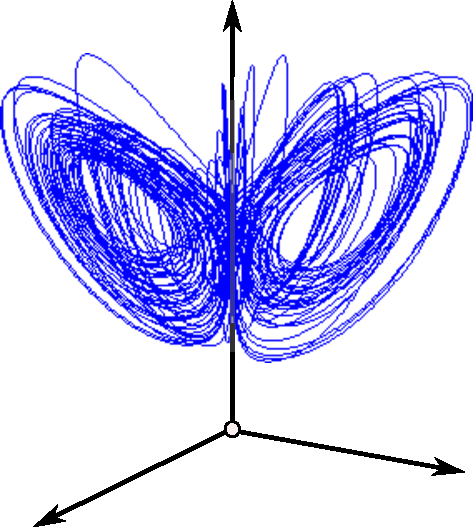
\includegraphics[width=\unitlength]{CLEattractor}}%
    	\put(0.55152995,1.0139628){\color[rgb]{0,0,0}\makebox(0,0)[lb]{\smash{$z$}}}%
    	\put(0.05573445,0.0739776){\color[rgb]{0,0,0}\makebox(0,0)[lb]{\smash{$x_1$}}}%
    	\put(0.90013492,0.16491708){\color[rgb]{0,0,0}\makebox(0,0)[lb]{\smash{$x_2$}}}%
  	\end{picture}%	
  (b)
  	\begin{picture}(1,1.06440474)%
    	\put(0,0){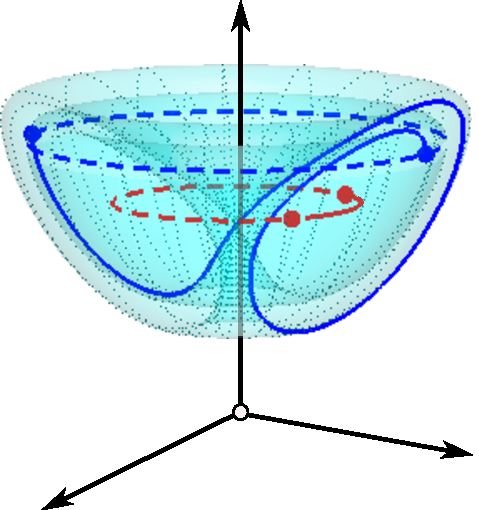
\includegraphics[width=\unitlength]{CLEWurst01}}%
   		\put(0.55961552,1.00214901){\color[rgb]{0,0,0}\makebox(0,0)[lb]{\smash{$z$}}}%
   		\put(0.07008555,0.07304272){\color[rgb]{0,0,0}\makebox(0,0)[lb]{\smash{$x_1$}}}%
    	\put(0.90381504,0.16283301){\color[rgb]{0,0,0}\makebox(0,0)[lb]{\smash{$x_2$}}}%
  	\end{picture}
\\
(c)   \begin{picture}(1,0.94310243)%
    \put(0,0){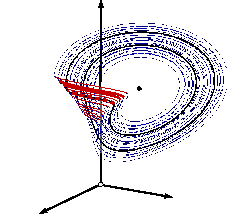
\includegraphics[width=\unitlength]{CLE1SliceSmall.pdf}}%
    \put(0.48564392,0.89244183){\color[rgb]{0,0,0}\makebox(0,0)[lb]{\smash{$z$}}}%
    \put(0.07181137,0.03185892){\color[rgb]{0,0,0}\makebox(0,0)[lb]{\smash{$y_2$}}}%
    \put(0.77031544,0.100183){\color[rgb]{0,0,0}\makebox(0,0)[lb]{\smash{$x_2$}}}%
  \end{picture}%
(d)   \begin{picture}(1,1.05662086)%
    \put(0,0){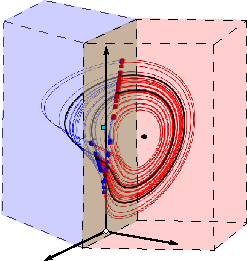
\includegraphics[width=\unitlength]{CLE2slicesmall.pdf}}%
    \put(0.47706962,0.83002768){\color[rgb]{0,0,0}\makebox(0,0)[lb]{\smash{$z$}}}%
    \put(0.08719004,0.02997825){\color[rgb]{0,0,0}\makebox(0,0)[lb]{\smash{$y_2$}}}%
    \put(0.73025395,0.09287946){\color[rgb]{0,0,0}\makebox(0,0)[lb]{\smash{$x_2$}}}%
  \end{picture}
    \end{center}
  \caption
  [\CLf: $\cycle{01}$ {\rpo} group orbit]{
  \CLf, $d=5 \to 3$~dimensional $\{x_1,x_2,z\}$ projections:
  (a)
  The strange attractor.
  (b)
  The initial \reqv\ $\REQV{}{1}$ point is shown by the red dot, and its
  group orbit / trajectory by the dashed red line. One period of the
  $\cycle{01}$ {\rpo} is shown by the solid blue line. The group orbit of
  its (arbitrary) starting point is shown by the dashed blue line: after
  one period the trajectory has returned to the group orbit but with a
  different phase. The \wurst, \ie, the group orbit of the $\cycle{01}$
  trajectory (dark blue) is shown by the cyan surface. Following
  $\cycle{01}$ for 15 more periods (faint dotted lines) starts filling
  out this torus; in that time the slowly drifting \reqv\ $\REQV{}{1}$
  has advanced to the next red dot (red line).
Symmetry-reduced \cLf, $d=4 \to 3$~dimensional $\{x_2,y_2,z\}$ projections:
 (c)
 Strange attractor (a) reduced to a single \slice\ hyperplane, using
 $\REQV{}{1}$ as the template. The dynamics exhibits singular jumps
 (shown in red) due to forbidden crossings of the \chartBord. In contrast
 to the 1\dmn\ \poincBord s of \reffig{fig:RoessTrjs}, here \chartBord s
 are 3\dmn\ and hard to visualize.
 (d)
The 2-chart atlas (sketched in \reffig{fig:A29-1ridge}) of the same
strange attractor encounters no \chartBord s and exhibits no
singularities. The ridge (shown in brown) acts as a \PoincSec\ $\PoincS$ with red or
blue ridge points $\sspRed^*$ marking the direction of the crossing.
  }
\label{fig:CLf01group}
\end{figure}
%%%%%%%%%%%%%%%%%%%%%%%%%%%%%%%%%%%%%%%%%%%%%%%%%%

 [blah blah]

 [blah blah]

\section{Chart}
\label{s:slice}

 [blah blah]

One can write the equations for the flow in the \reducedsp\
$\dot{\sspRed} = \velRed(\sspRed)$ (for details see, for example,
\refref{DasBuch}) as
\bea
\velRed(\sspRed) &=& \vel(\sspRed)
     \,-\, \dot{\gSpace}(\sspRed) \, \groupTan(\sspRed)
\label{2modesEqMotMFrame}\\
\dot{\gSpace}(\sspRed) &=& \braket{\vel(\sspRed)}{\sliceTan{}}
                       /\braket{\groupTan(\sspRed)}{\sliceTan{}}
\,
\label{2modesreconstrEq}
\eea
which confines the motion to the \slice\ hyperplane. Thus, the dynamical
system $\{\pS,\map^t\}$ with continuous symmetry \Group\ is replaced by
the {\reducedsp} dynamics $\{\pSRed,\mapRed^t\}$: The velocity in the
full \statesp\ $\vel$ is the sum of $\velRed$, the velocity component in
the \slice\ hyperplane, and $\dot{\gSpace}\,\groupTan$, the velocity
component along the group tangent space. The integral of the {\em
reconstruction equation} for $\dot{\gSpace}$ keeps track of the group
shift in the full \statesp.


 [blah blah]

\section{Charting the \slice}
\label{s:chart}

Let us summarize the voyage so far:

 [blah blah]


How the charts are put together is best told as a graphic tale, in the 5
frames of Figs.  [blah blah]



\section{Conclusions}
\label{s:concl}

 [blah blah]

\begin{acknowledgments}
This article addresses the questions asked after the  [blah blah]
We are indebted to
 [blah blah]
and
 [blah blah]
for inspiring discussions.
\end{acknowledgments}


\bibliography{../bibtex/siminos}


\ifdraft
    \onecolumngrid

    \newpage
\input flotsam
    \newpage
    \section{Daily blog, point by point}
    \label{chap:atlas}
\input ../blog/atlas
\fi

\end{document}
